\documentclass[12pt]{article}
\usepackage[a4paper,margin=1in]{geometry}
\usepackage{titling}
\usepackage[utf8]{inputenc}
\usepackage{graphicx}
\usepackage{xcolor}
\usepackage{listings}
\usepackage{amsmath}
\usepackage{geometry}
\geometry{margin=1in}
\setlength{\parskip}{0em}
\lstset{
    backgroundcolor=\color{blue!2},
    basicstyle=\ttfamily\small,
    frame=single,
    breaklines=true,
    keywordstyle=\color{blue},
    commentstyle=\color{green!50!black}
}


\begin{document}

\begin{titlepage}
    \centering
    \vspace*{\fill}

    {\Large\textbf{Parallel Programming for High-Performance Computing}}\\
    (PPAR, MU4IN903)

    \vspace{1cm}

    {\Large\textbf{Sorbonne University}}

    \vspace{5cm}

    {\large\textbf{Golden Collision by the "MitM Attack"}}

    \vspace{1cm}

    {\large\textbf{By}}

    \vspace{1cm}

    {\Large Matthieu Bidault - (ID: 21401573)}\\
    {\Large Houssam Nasser - (ID: 21400407)}

    \vspace*{\fill}
\end{titlepage}

\newpage
\section*{Parallelization of the Direct MITM Attack}

\begin{figure}[htp]
    \centering
    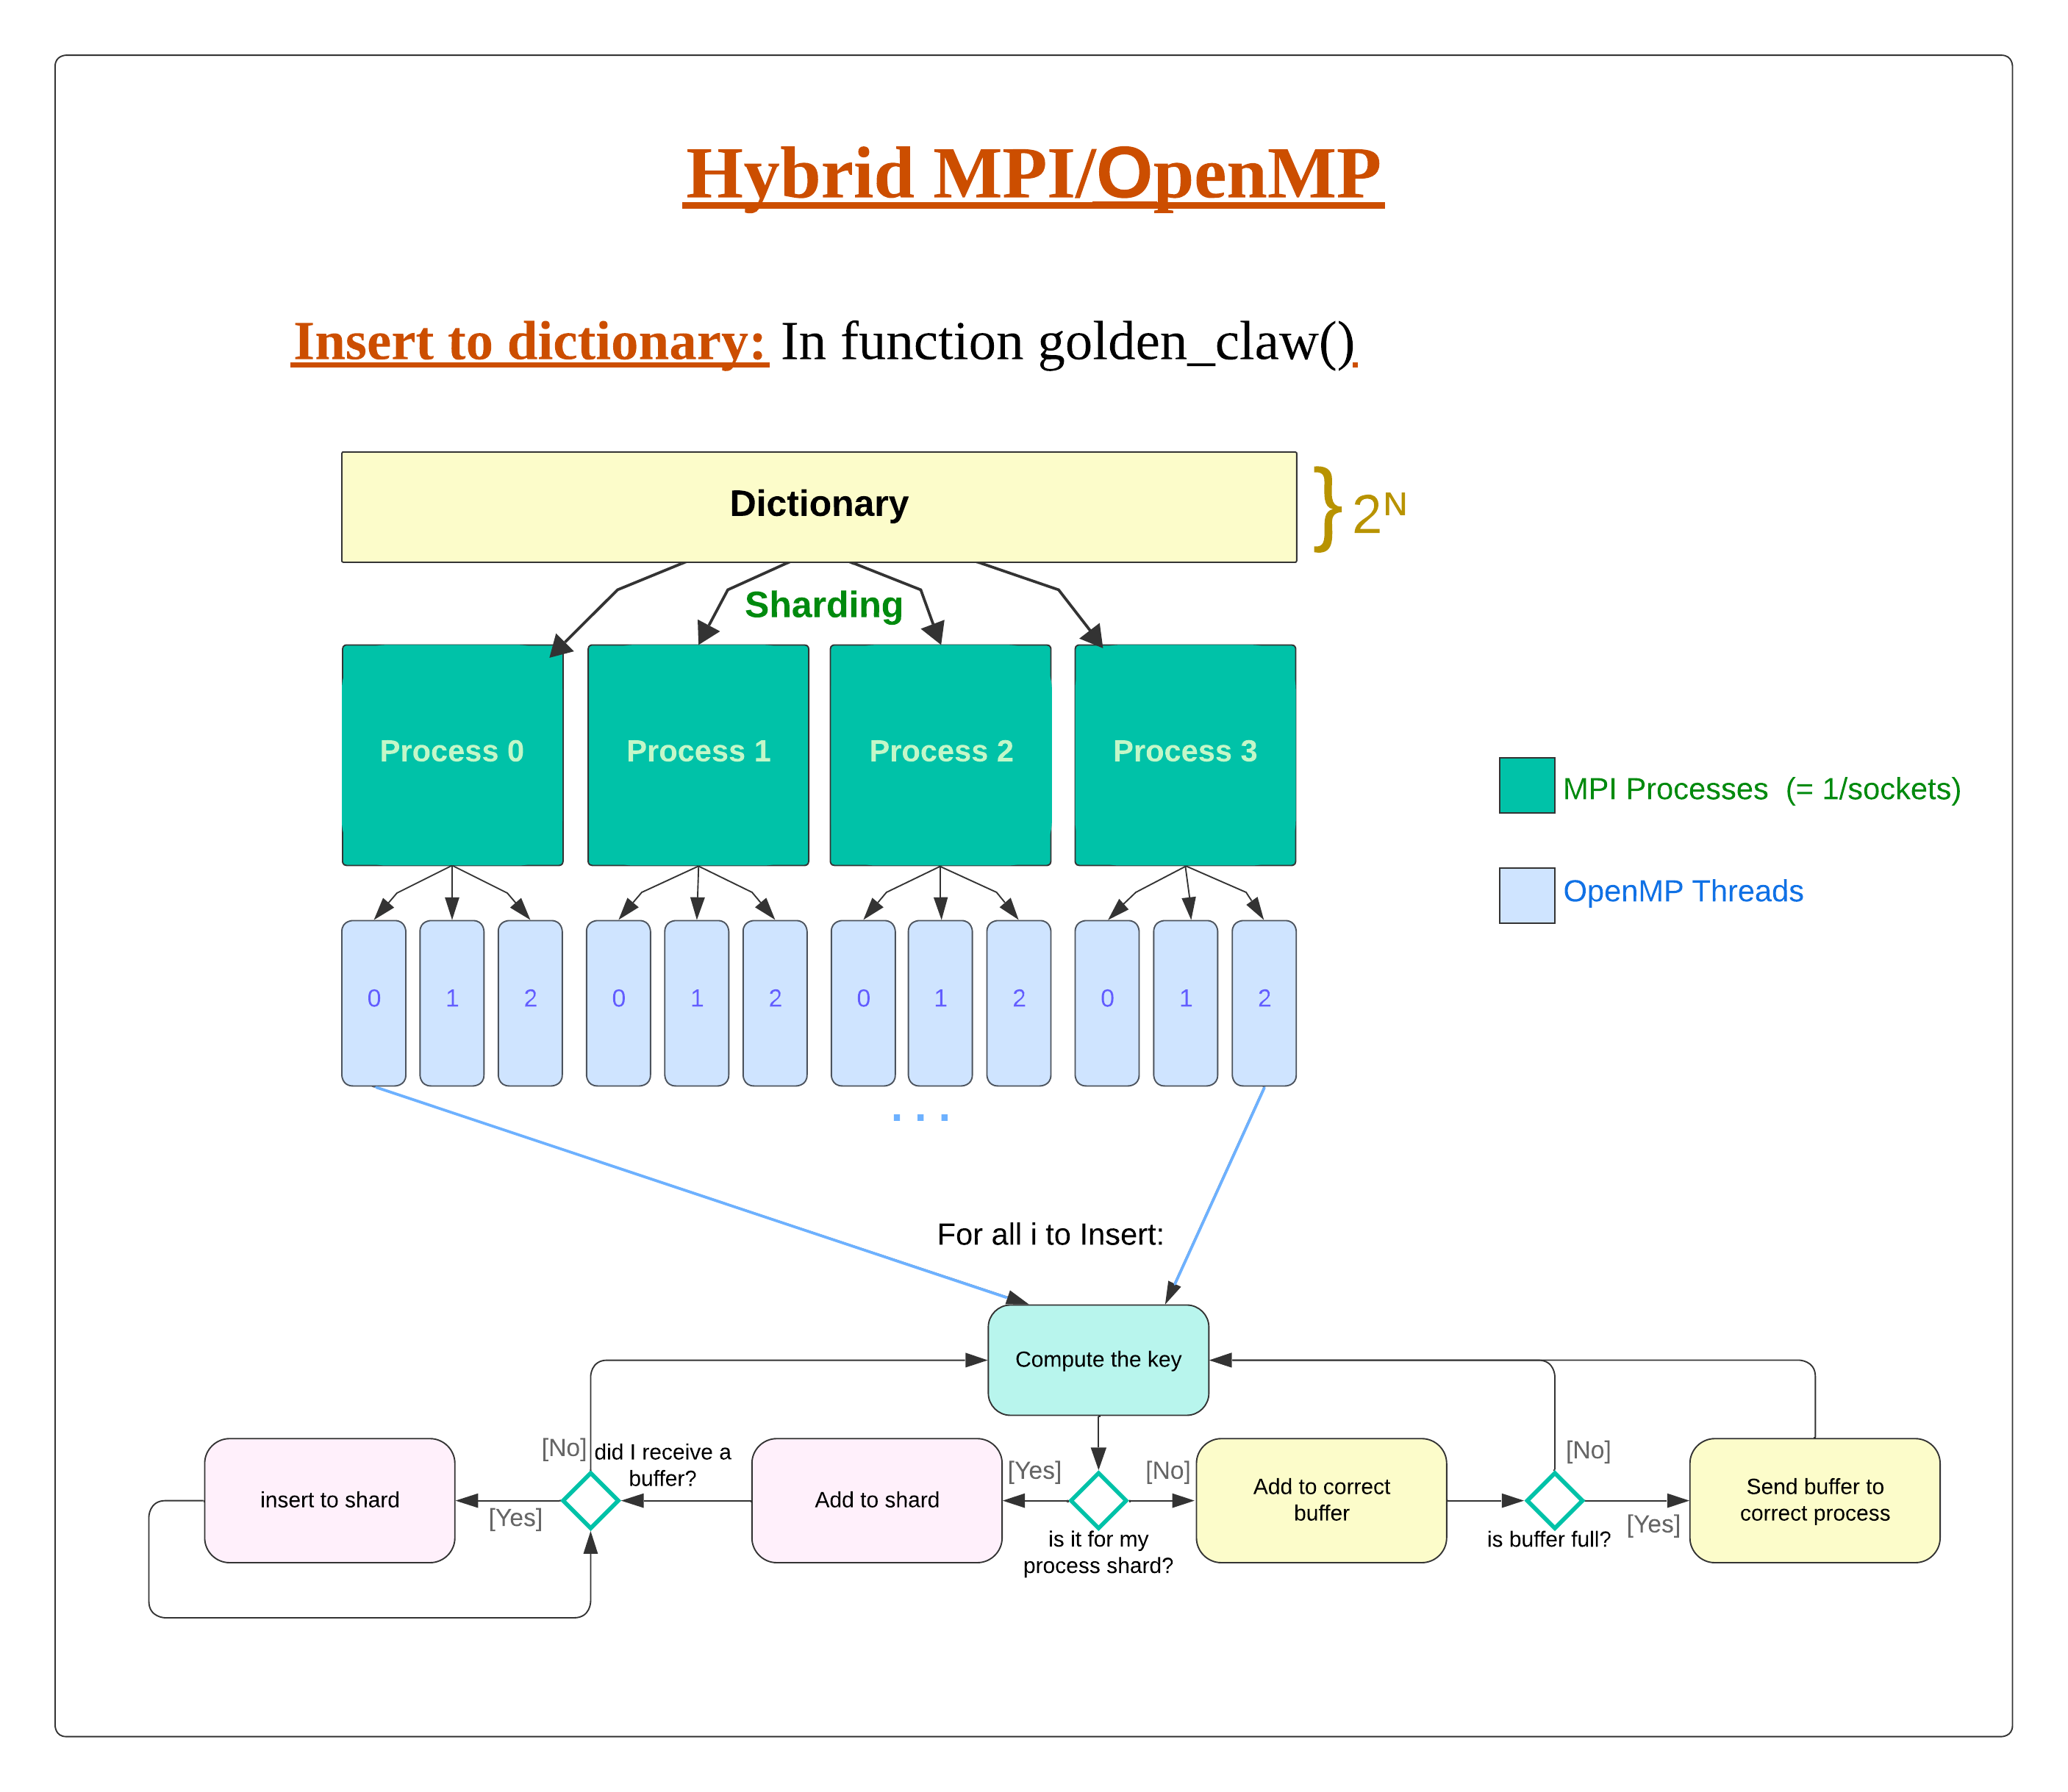
\includegraphics[width=15cm]{Copy of Copy of Activity diagram33 (2).png}
    \caption{Hybrid Parallelization Scheme}
\end{figure}

The parallelization strategy is based on distributing the dictionary into shards across multiple MPI processes and further parallelizing computations within each process using OpenMP threads. The diagram illustrates this as follows:

\begin{enumerate}
    \item \textbf{Sharding:} The dictionary, representing a $2^N$ key space, is divided among MPI processes based on their rank.
    \item \textbf{Buffering and Insertion:}
        \begin{itemize}
            \item Each MPI process computes keys and decides if a key belongs to its shard.
            \item If the key belongs to another process's shard, it is added to a buffer and sent when the buffer is full.
            \item Each process receives buffers from others and inserts keys into its local shard.
        \end{itemize}
    \item \textbf{Thread-Level Parallelism:} Each process utilizes OpenMP threads to parallelize key computation, buffer management, and insertion tasks.
\end{enumerate}

\section*{Parallelization Details}

\subsection*{MPI Implementation}
MPI handles inter-process communication and sharding. Key functions include:

\begin{itemize}
    \item \textbf{MPI\_Send} and \textbf{MPI\_Recv}: Used to send and receive buffers of keys between processes.
    \item \textbf{MPI\_Allreduce}: Ensures global synchronization and checks if a solution has been found.
\end{itemize}

\begin{lstlisting}[language=C]
MPI_Send(buffers[i], buffer_size * 2, MPI_UINT64_T, i, TO_INSERT_TAG, MPI_COMM_WORLD);
MPI_Recv(buffers[mpi_rank], buffer_size * 2, MPI_UINT64_T, rank, TO_INSERT_TAG, MPI_COMM_WORLD, &status);
MPI_Allreduce(&nres, &global_nres, 1, MPI_INT, MPI_SUM, MPI_COMM_WORLD);
\end{lstlisting}

\subsection*{OpenMP Implementation}
OpenMP is used for intra-process parallelism. Key constructs include:

\begin{itemize}
    \item \textbf{\#pragma omp parallel for}: Distributes the computation of keys across threads.
    \item \textbf{\#pragma omp atomic}: Ensures thread-safe updates to shared data structures, such as buffer indices.
\end{itemize}

\begin{lstlisting}[language=C]
#pragma omp parallel for schedule(static)
for (u64 x = mpi_rank; x < N; x += mpi_size) {
    u64 z = f(x);
    int r = z % mpi_size;
    if (r == mpi_rank) {
        dict_insert(z, x);
    } else {
        u64 index;
#pragma omp atomic capture
        index = buffer_idx[r]++;
        buffers[r][index * 2] = x;
        buffers[r][index * 2 + 1] = z;
    }
}
\end{lstlisting}

    \vspace{0.5cm}

By combining MPI for process-level distribution and OpenMP for thread-level parallelism, the program effectively utilizes cluster resources. This hybrid approach achieves significant scalability by Maximizing CPU core utilization via multi-threaded computations within each process.

The use of hybrid MPI/OpenMP significantly reduces computation time, allowing for the handling of large key spaces (e.g., $N \geq 37$).

\newpage

\section*{Performance Analysis}
% Commands Section
The following commands were used to execute the tests on different clusters and configurations:
\begin{lstlisting}[language=bash, basicstyle=\ttfamily\footnotesize, backgroundcolor=\color{gray!10}]
./mitm --n 20 --C0 6184c52d0df0137a --C1 915d64a00528cfc0
./mitm --n 31 --C0 8f382b169e3ef269 --C1 a4e74e0ceb927493
./mitm --n 32 --C0 9dd43cc240131938 --C1 03a38ed28e9e6171
./mitm --n 35 --C0 baf19ec5610866cb --C1 7e074786450ee37f
./mitm --n 37 --C0 be9a6fc43423c485 --C1 789d8c2530c54c8d
./mitm --n 40 --C0 70e20a208dd9a4ee --C1 22b9c07cffb0fae1
./mitm --n 42 --C0 46da2c4e8d8d7705 --C1 5da937a1279f80f6
\end{lstlisting}

\subsection*{Tests on 30 nodes at Nantes (60 processes, 600 cores)}
The line graph below illustrates the execution time for different configurations and input sizes on the Nantes cluster.

\begin{figure}[h!]
    \centering
    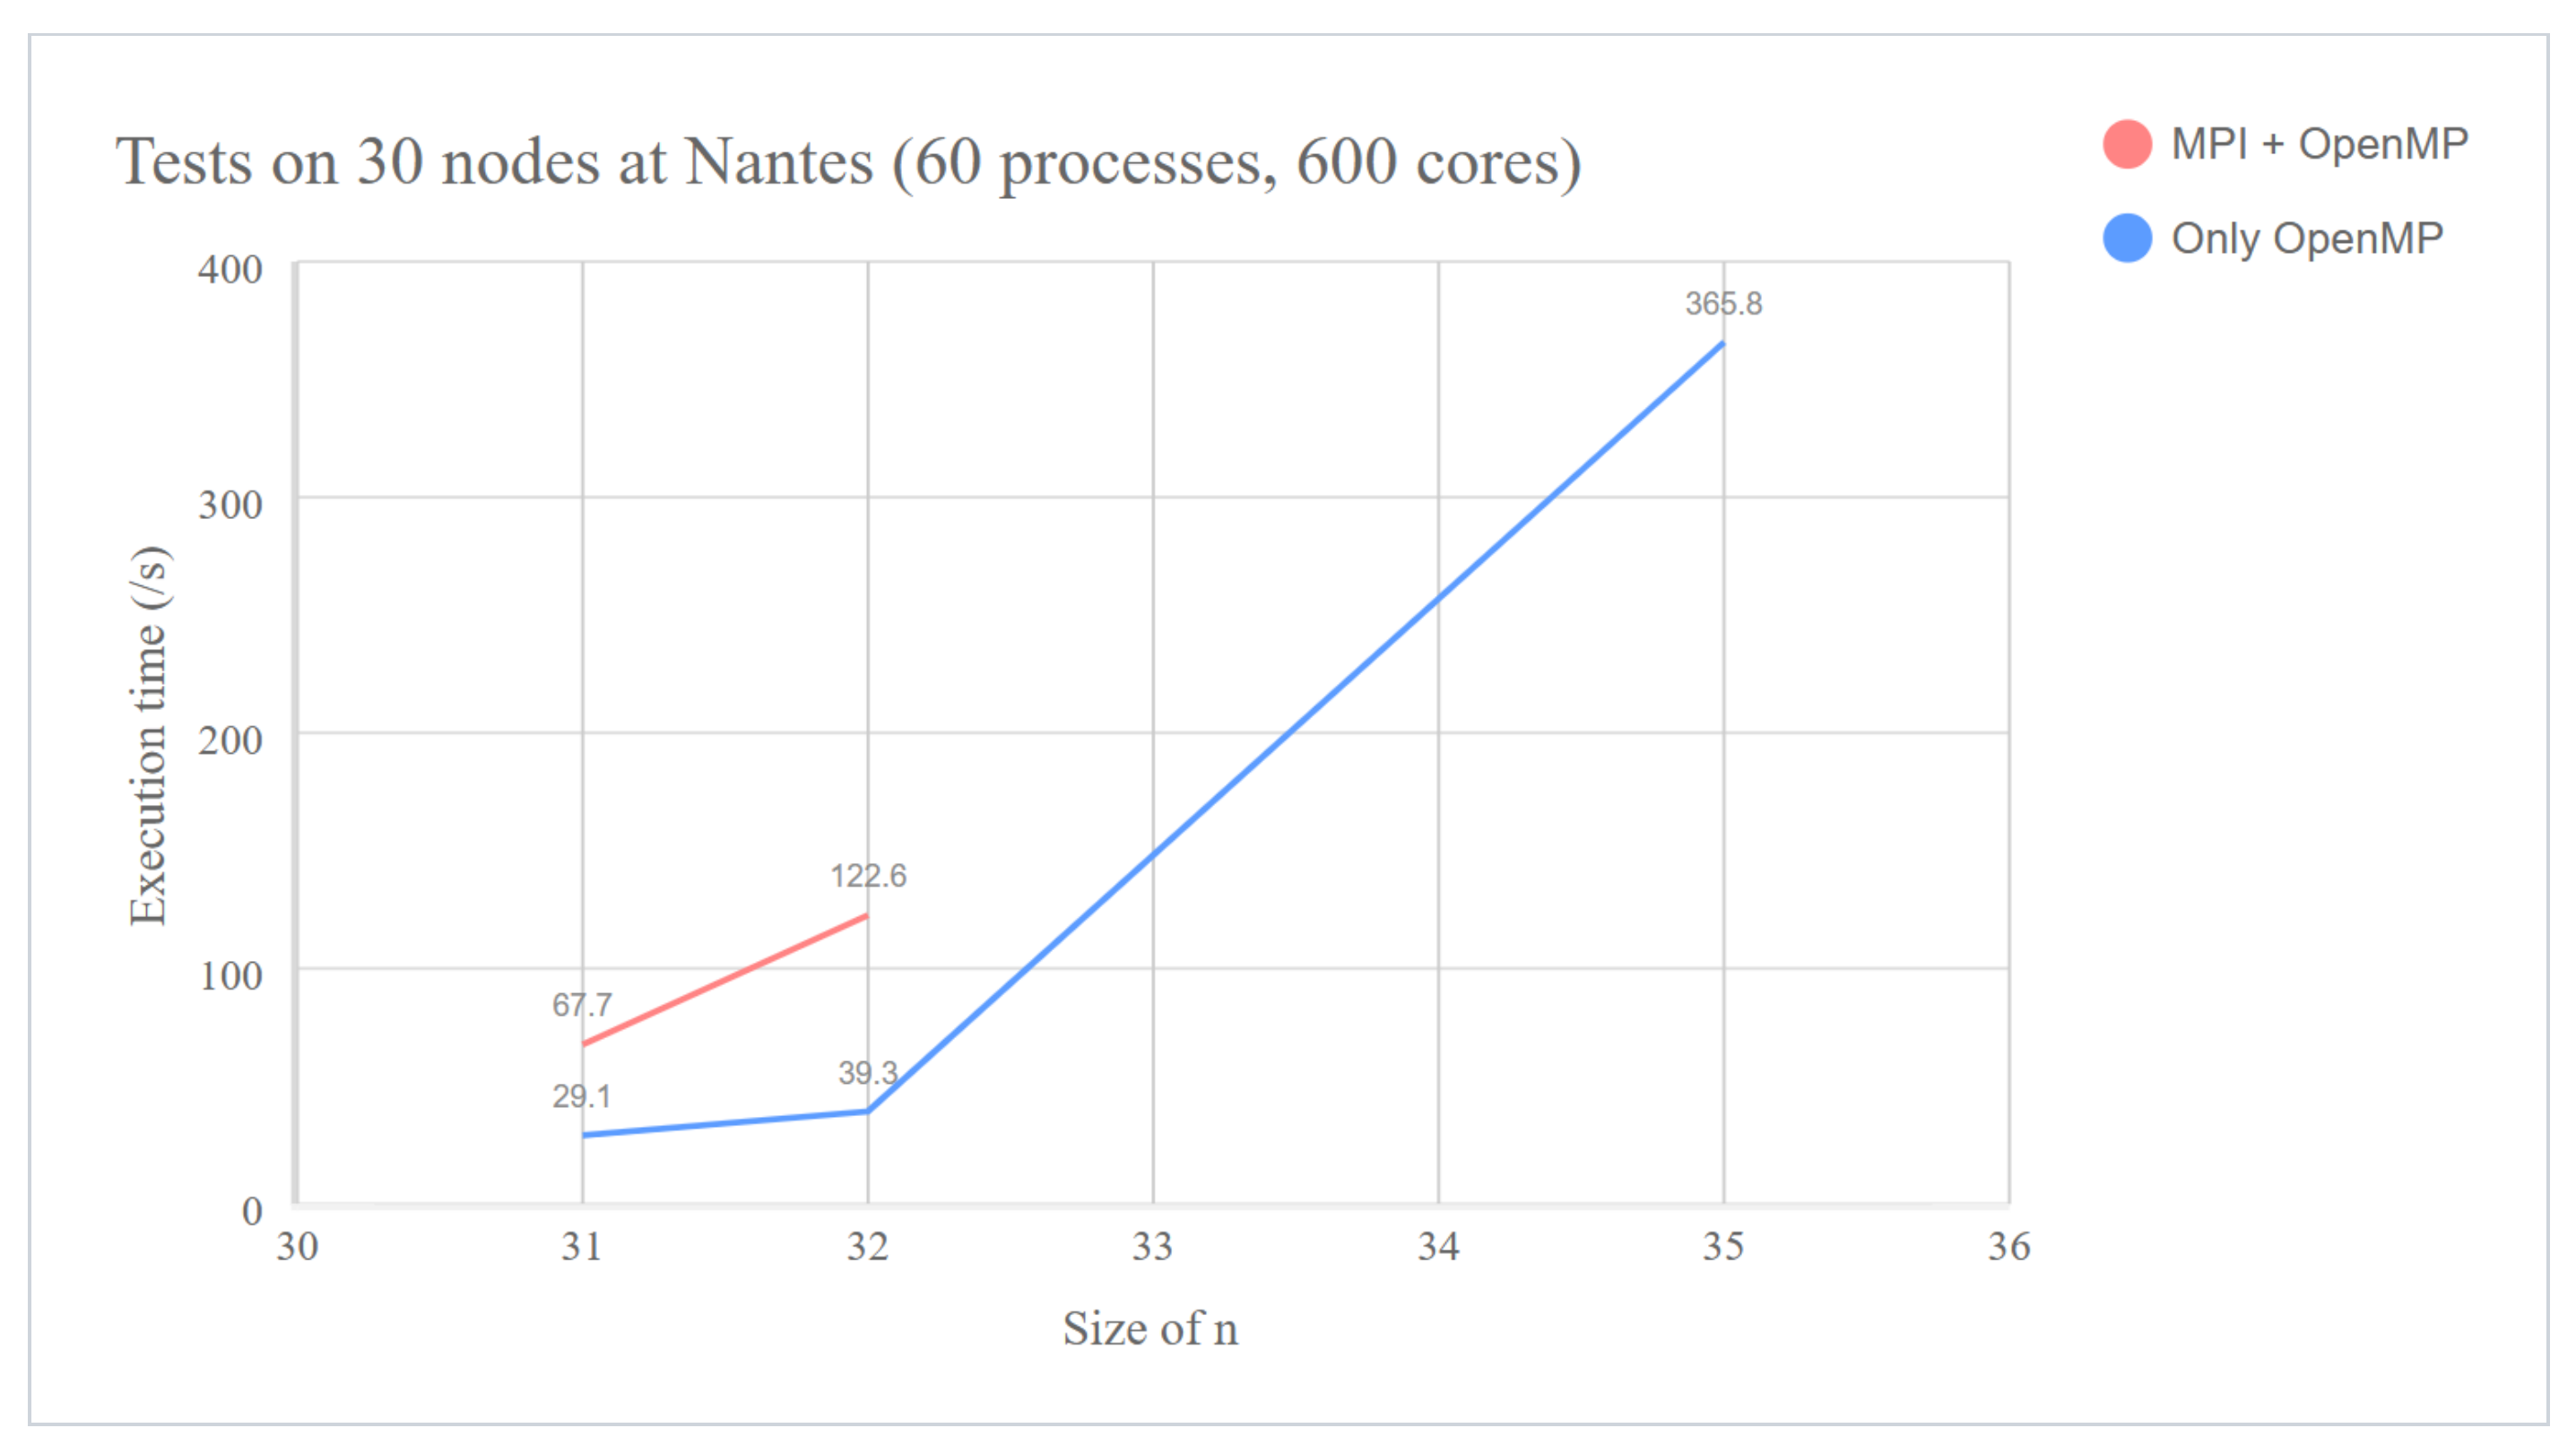
\includegraphics[width=1\linewidth]{tests on 30 nodes at Nantes (60 processes, 600 cores) (2).png}
    \caption{Execution time on 30 nodes at Nantes}
\end{figure}

In this configuration:

- \textbf{Only MPI}: was not tested for smaller inputs but was slower compared to the hybrid approach for larger inputs.

- \textbf{Only OpenMP}: showed impressive results for smaller problem sizes due to reduced inter-process communication overhead but scaled poorly for larger sizes.

- \textbf{MPI + OpenMP}: achieved the best balance for moderate problem sizes by utilizing intra-node and inter-node parallelism effectively.

\vspace{0.5cm}

\textbf{Speedup:} For $n=32$, comparing OpenMP only (39.37s) to MPI+OpenMP (122.6s), the speedup was 39.37/122.6 = 0.32. The hybrid approach was efficient for larger problem sizes but had a higher communication overhead for smaller sizes.


\subsection*{Tests on 55 gros nodes in Nancy (990 cores)}
The line graph below demonstrates the performance in Nancy's cluster.
 
\begin{figure}[h!]
    \centering
    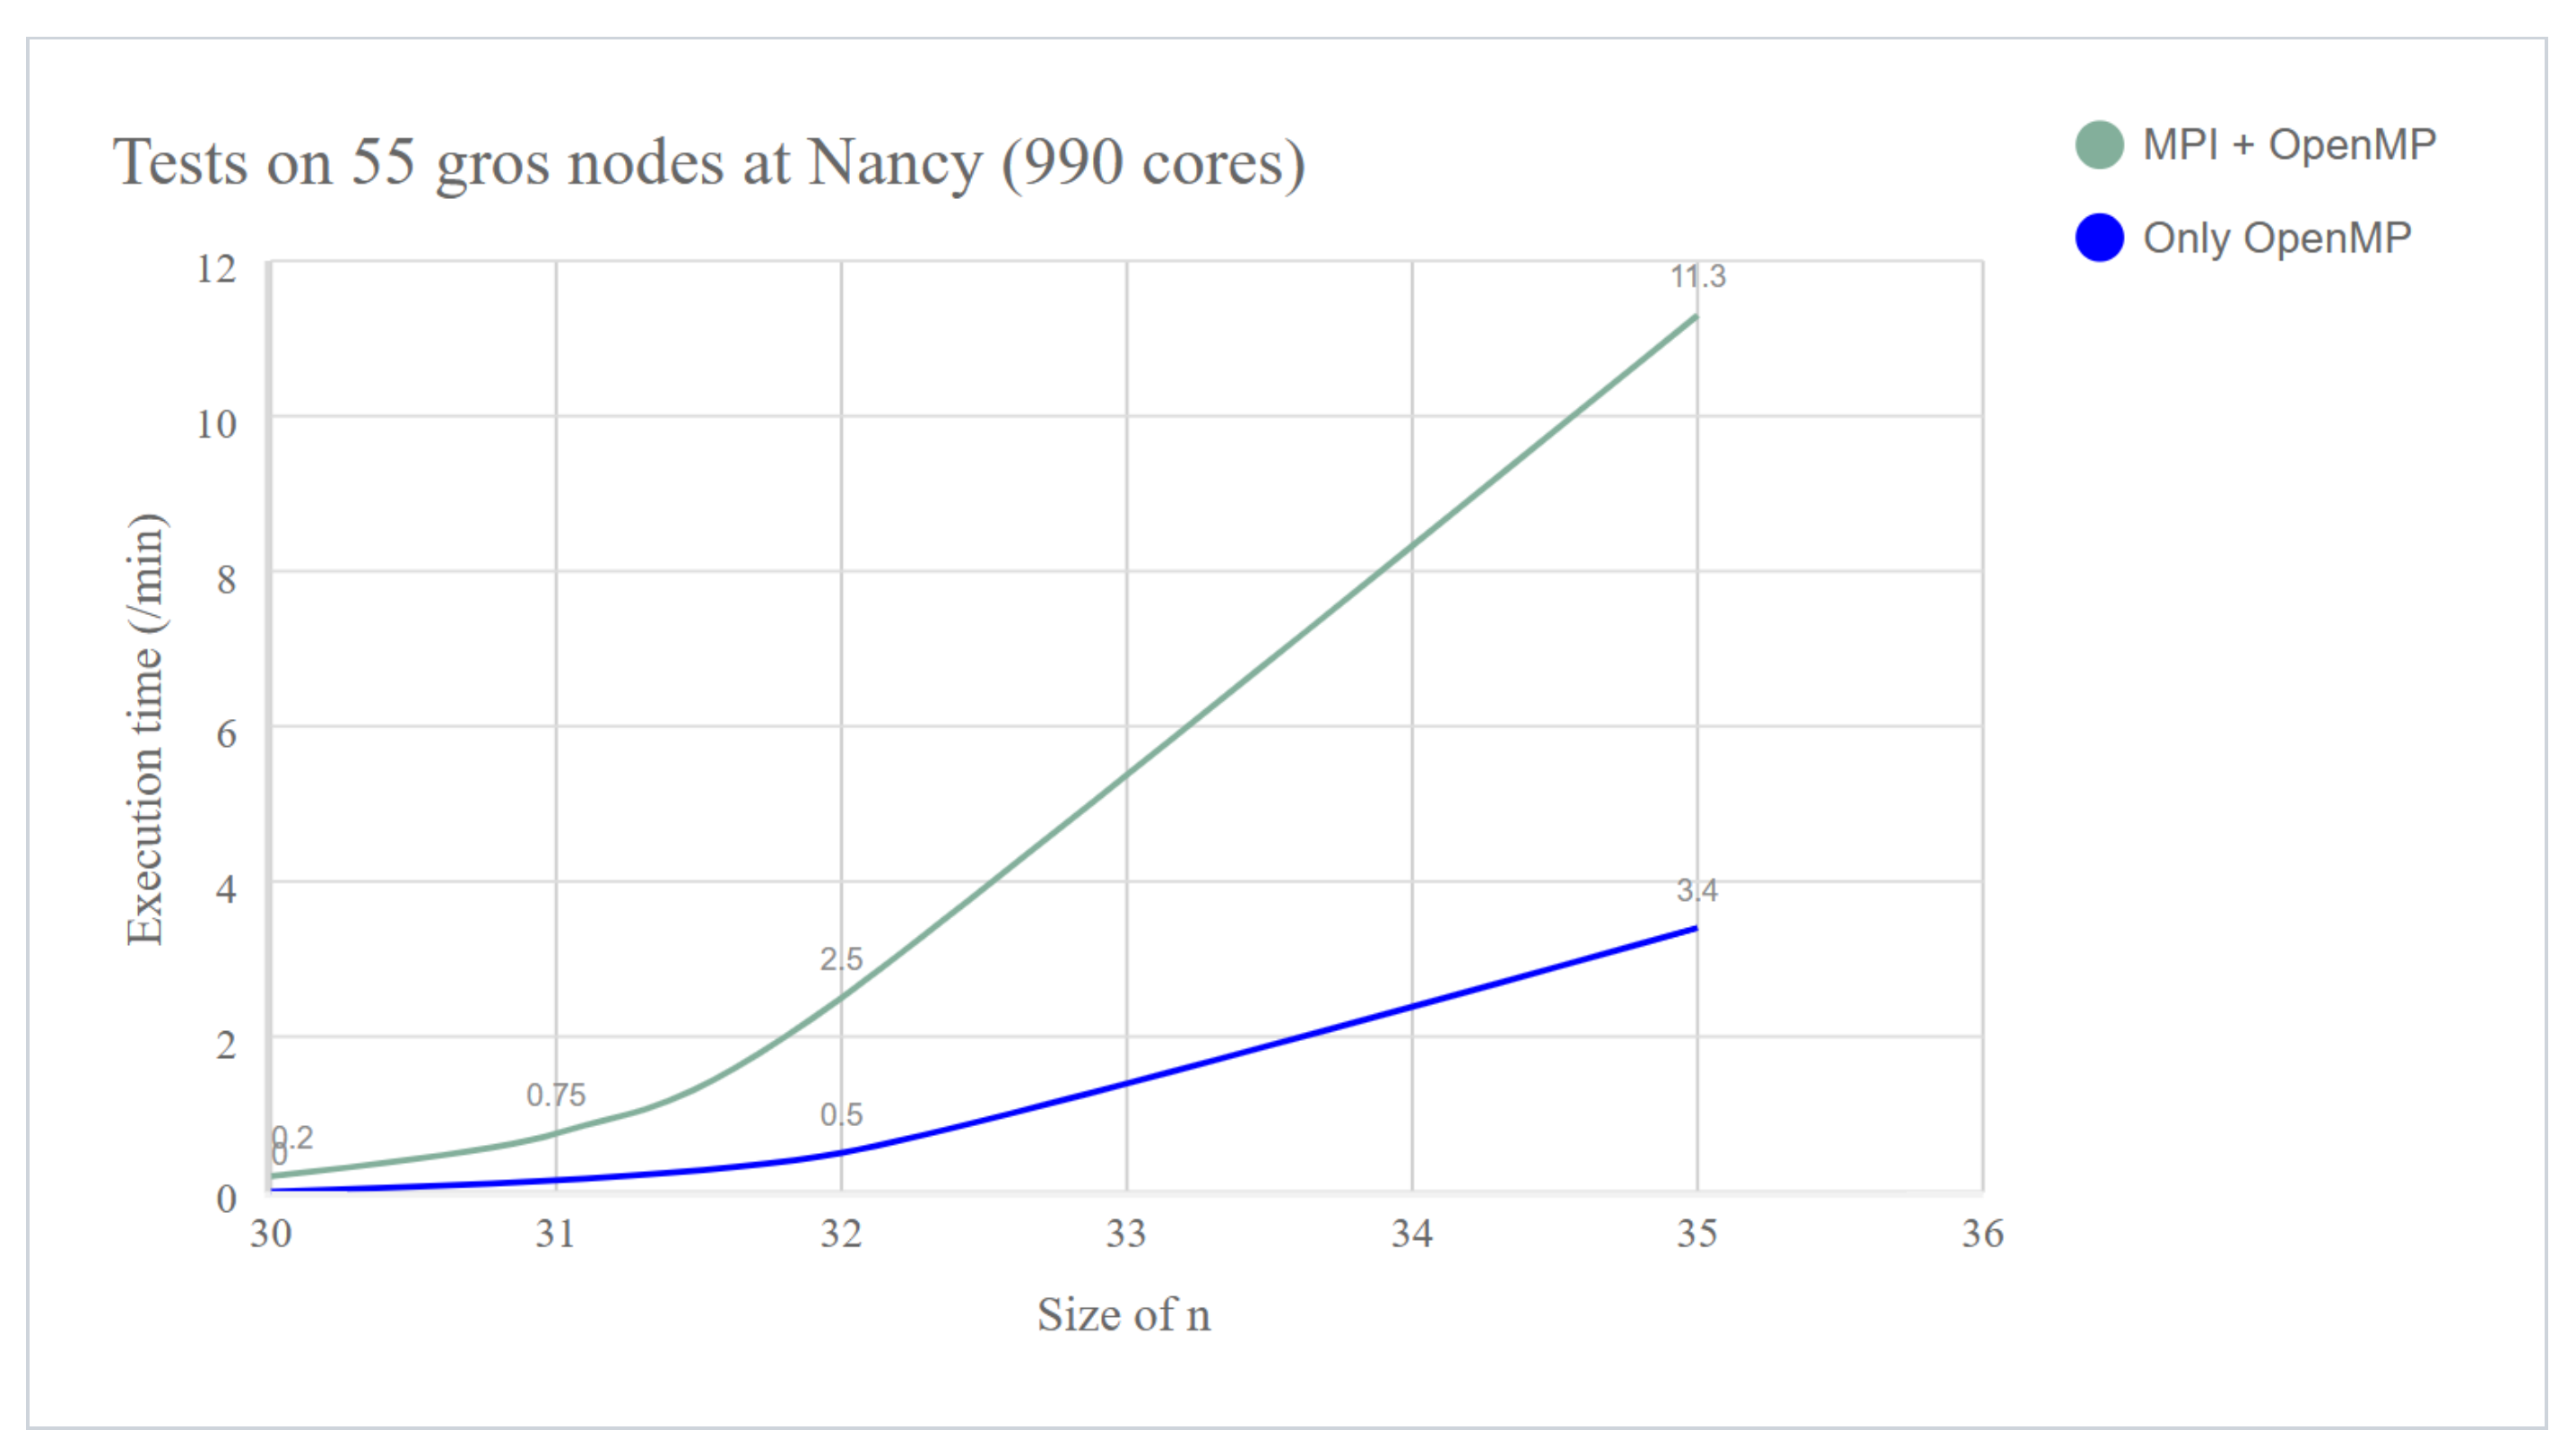
\includegraphics[width=1.1\linewidth]{tests on 55 gros nodes at Nancy (990 cores) (2).png}
    \caption{Execution time on 55 gros nodes at Nancy }
\end{figure}


\vspace{1cm}

For Nancy:

- \textbf{MPI + OpenMP}: showed consistent performance for all tested sizes, leveraging the large number of cores available.

- \textbf{Only OpenMP}: was faster due to the lack of MPI communication.

\vspace{1cm}

\textbf{Speedup:} For $n=35$, OpenMP only (3.4 min) outperformed the hybrid approach (11.3 min). Speedup = 3.4/11.3 = 0.3.

\newpage

\subsection*{Tests on 15 paradoxe nodes in Rennes}
The results for Rennes are presented in the graph below.

\begin{figure}[h!]
    \centering
    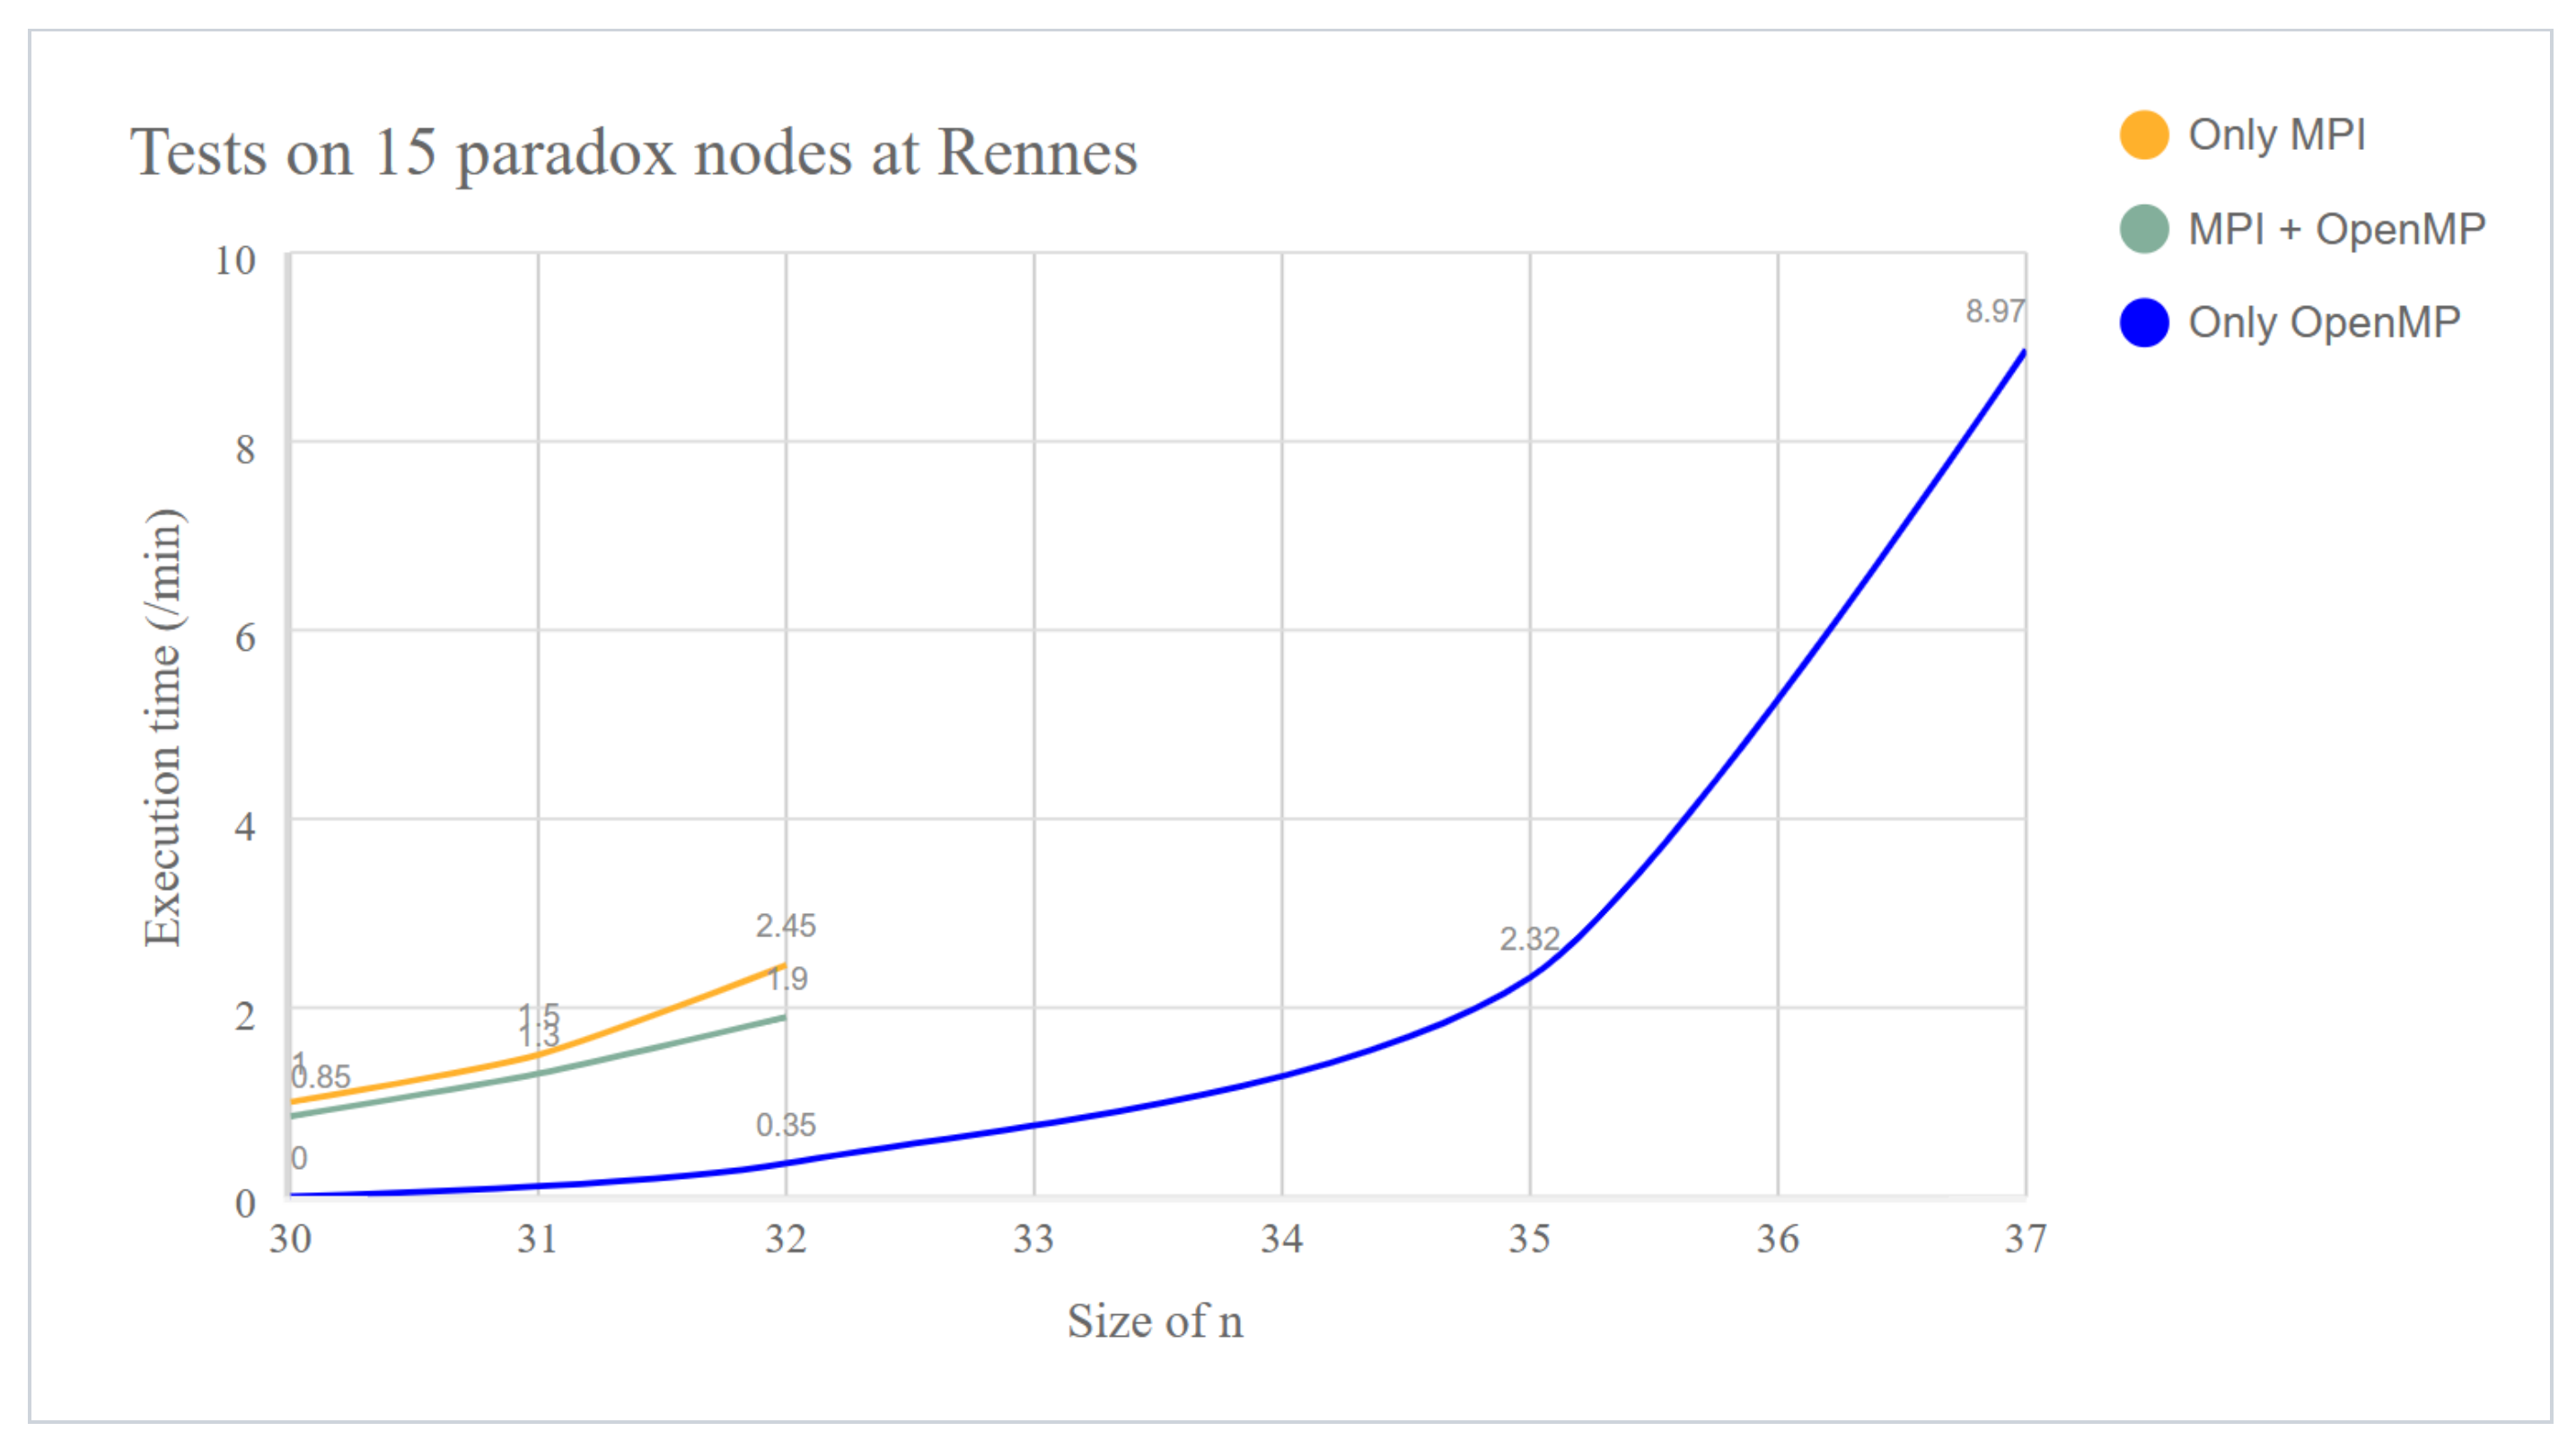
\includegraphics[width=1.11\linewidth]{tests on 15 paradoxe nodes at Rennes (2).png}
    \caption{Execution time on 15 paradoxe nodes at Rennes}
\end{figure}


On the Rennes cluster:

- \textbf{Only MPI}: showed slower performance due to limited optimization of intra-node parallelism.

- \textbf{Only OpenMP}: performed best for small problem sizes, but scaled poorly beyond $n=35$.

- \textbf{MPI + OpenMP}: was the most effective for $n>32$, leveraging both inter-node and intra-node optimizations.

\vspace{0.3cm}

\textbf{Speedup:} Comparing OpenMP only (0.35 min) with MPI + OpenMP (1.9 min) for $n=32$, the speedup was minimal. However, for $n=37$, the hybrid approach demonstrated much better scaling.

\section*{Summary of Observations}
1. \textbf{Hybrid MPI+OpenMP} achieved the best performance for larger input sizes.

2. \textbf{Only OpenMP} performed well for smaller sizes, but lacked scalability.

3. \textbf{Only MPI} was consistently slower due to lack of intranode parallel optimization.

\vspace{0.5cm}

\textbf{Conclusion:} The hybrid parallelization approach effectively utilized the available resources, achieving balanced performance for both small and large inputs. However, the trade-off between communication overhead and computation must be carefully balanced to optimize execution times.
























\end{document}
